
\chapter{Generalization of Algorithm}
\label{chap:application_krebs}


In this chapter, the insights obtained from the \gls{ILS} algorithm and its classifier-based variants are extended by
applying them to instances from the \krebsADataSetText dataset (see Section~\ref{fig:dataset_comparison}). Building on
the previous findings, two complementary approaches are investigated. The first approach generates training datasets
directly from the \krebsADataSetText instances, whereas the second employs pretrained classifiers derived from the
\gendreauDataSetText dataset.
Out of the 600 published instances, 50 were randomly selected for evaluation (Section~\ref{sec:dataset_selection}).
The procedures corresponding to each approach are described in Sections~\ref{sec:krebs_data_retrieval} and
\ref{sec:krebs_data_pretrained_models}. The comparative results are presented in Section~\ref{sec:results_krebs},
providing insights as to whether the generalization can be considered successful.


\section{Dataset Retrieval}
\label{sec:krebs_data_retrieval}

This section presents the training data retrieved with the save and random strategy (see Section~\ref{sec:DataRetrieval}). Furthermore,
the training datasets are analyzed and compared to the training datasets of \gendreauDataSet. Subsequently, one dataset is selected by
comparing the cross performance metrics of all datasets, similar to the procedure presented in Section~\ref{sec:dataset_selection}, but no
validation dataset is constructed.

\subsubsection{Random retrieval strategy}
The solvation of an average route, is significantly more challenging, as the number of items and customers is higher than for the
\gendreauDataSetText (see Section~\ref{fig:dataset_comparison}). Therefore, the following random datasets contain less routes and are presented in
the next Table~\ref{tab:random_instances_krebs}.
\begin{table}[ht]
    \centering
    \begin{tabular}{l c c c c c }
        \toprule
        Name        & Routes & Routes Len = 2 & Balance   & Rel. Vol & Rel. Mass \\
        \midrule
        RD-1-1-1-6  & 4836   & 92             & 75.3/24.7 & 0.30     & 0.52      \\
        RD-1-1-1-8  & 6099   & 94             & 69.7/30.3 & 0.33     & 0.57      \\
        RD-1-1-1-10 & 6707   & 80             & 64.9/35.1 & 0.37     & 0.63      \\

        \bottomrule
    \end{tabular}
    \caption{Random strategy train datsets from \krebsADataSet.}
    \label{tab:random_instances_krebs}
\end{table}
More insights about the computational challenges, classifiying the random datasets and an comparison to the \gendreauDataSetText is presented
in Subsection~\ref{subsec:challenges_krebs_random}. Generally, the balance between feasible and infeasible instances is reversed
compared to the random datasets shown in Table~\ref{tab:created_instances_xyz_gendreau}, while the relative volume of tours
is considerably smaller. This effect can be attributed to the small parameter values of the \gls{RRG} algorithm ($\alpha$, $\beta$, $\gamma$),
which cause the algorithm to terminate more quickly. However, the average number of
customers per route is approximately doubled (see next Figure~\ref{fig:route_cust_no_krebs_new}).

\begin{figure}[ht]
    \centering
    \begin{subfigure}[t]{.5\textwidth}
        \centering
        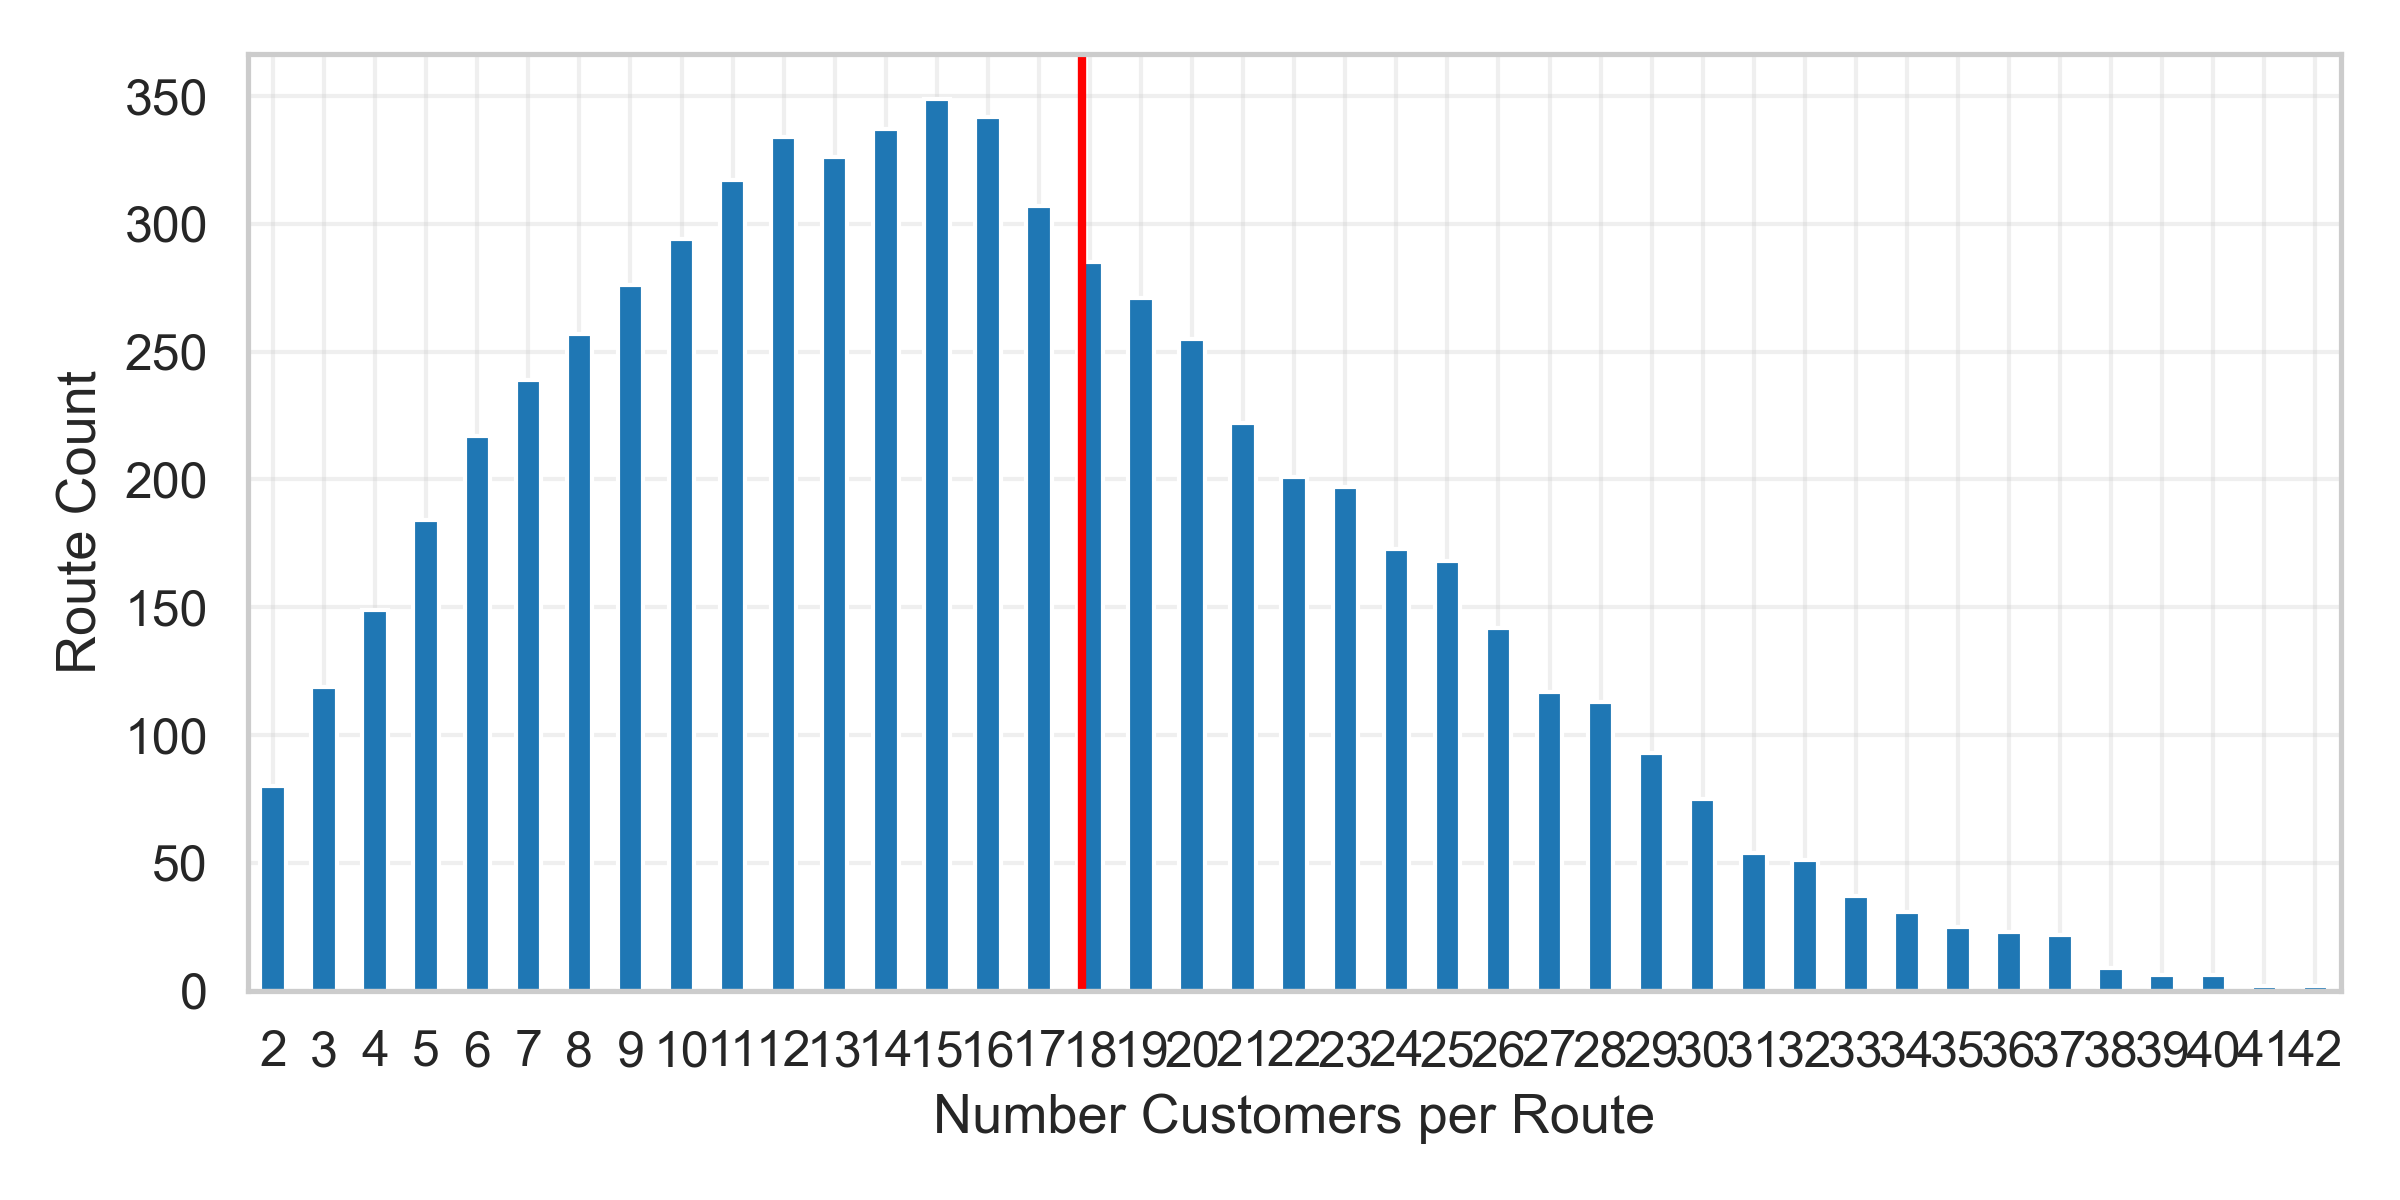
\includegraphics[width=\linewidth]{pictures/dataset_structure/no_cust_plot_RandomData_1_1_1_10.png}
        \caption{Dataset RD-1-1-1-10}
        \label{fig:ds-a-krebs_lop}
    \end{subfigure}%
    \begin{subfigure}[t]{.5\textwidth}
        \centering
        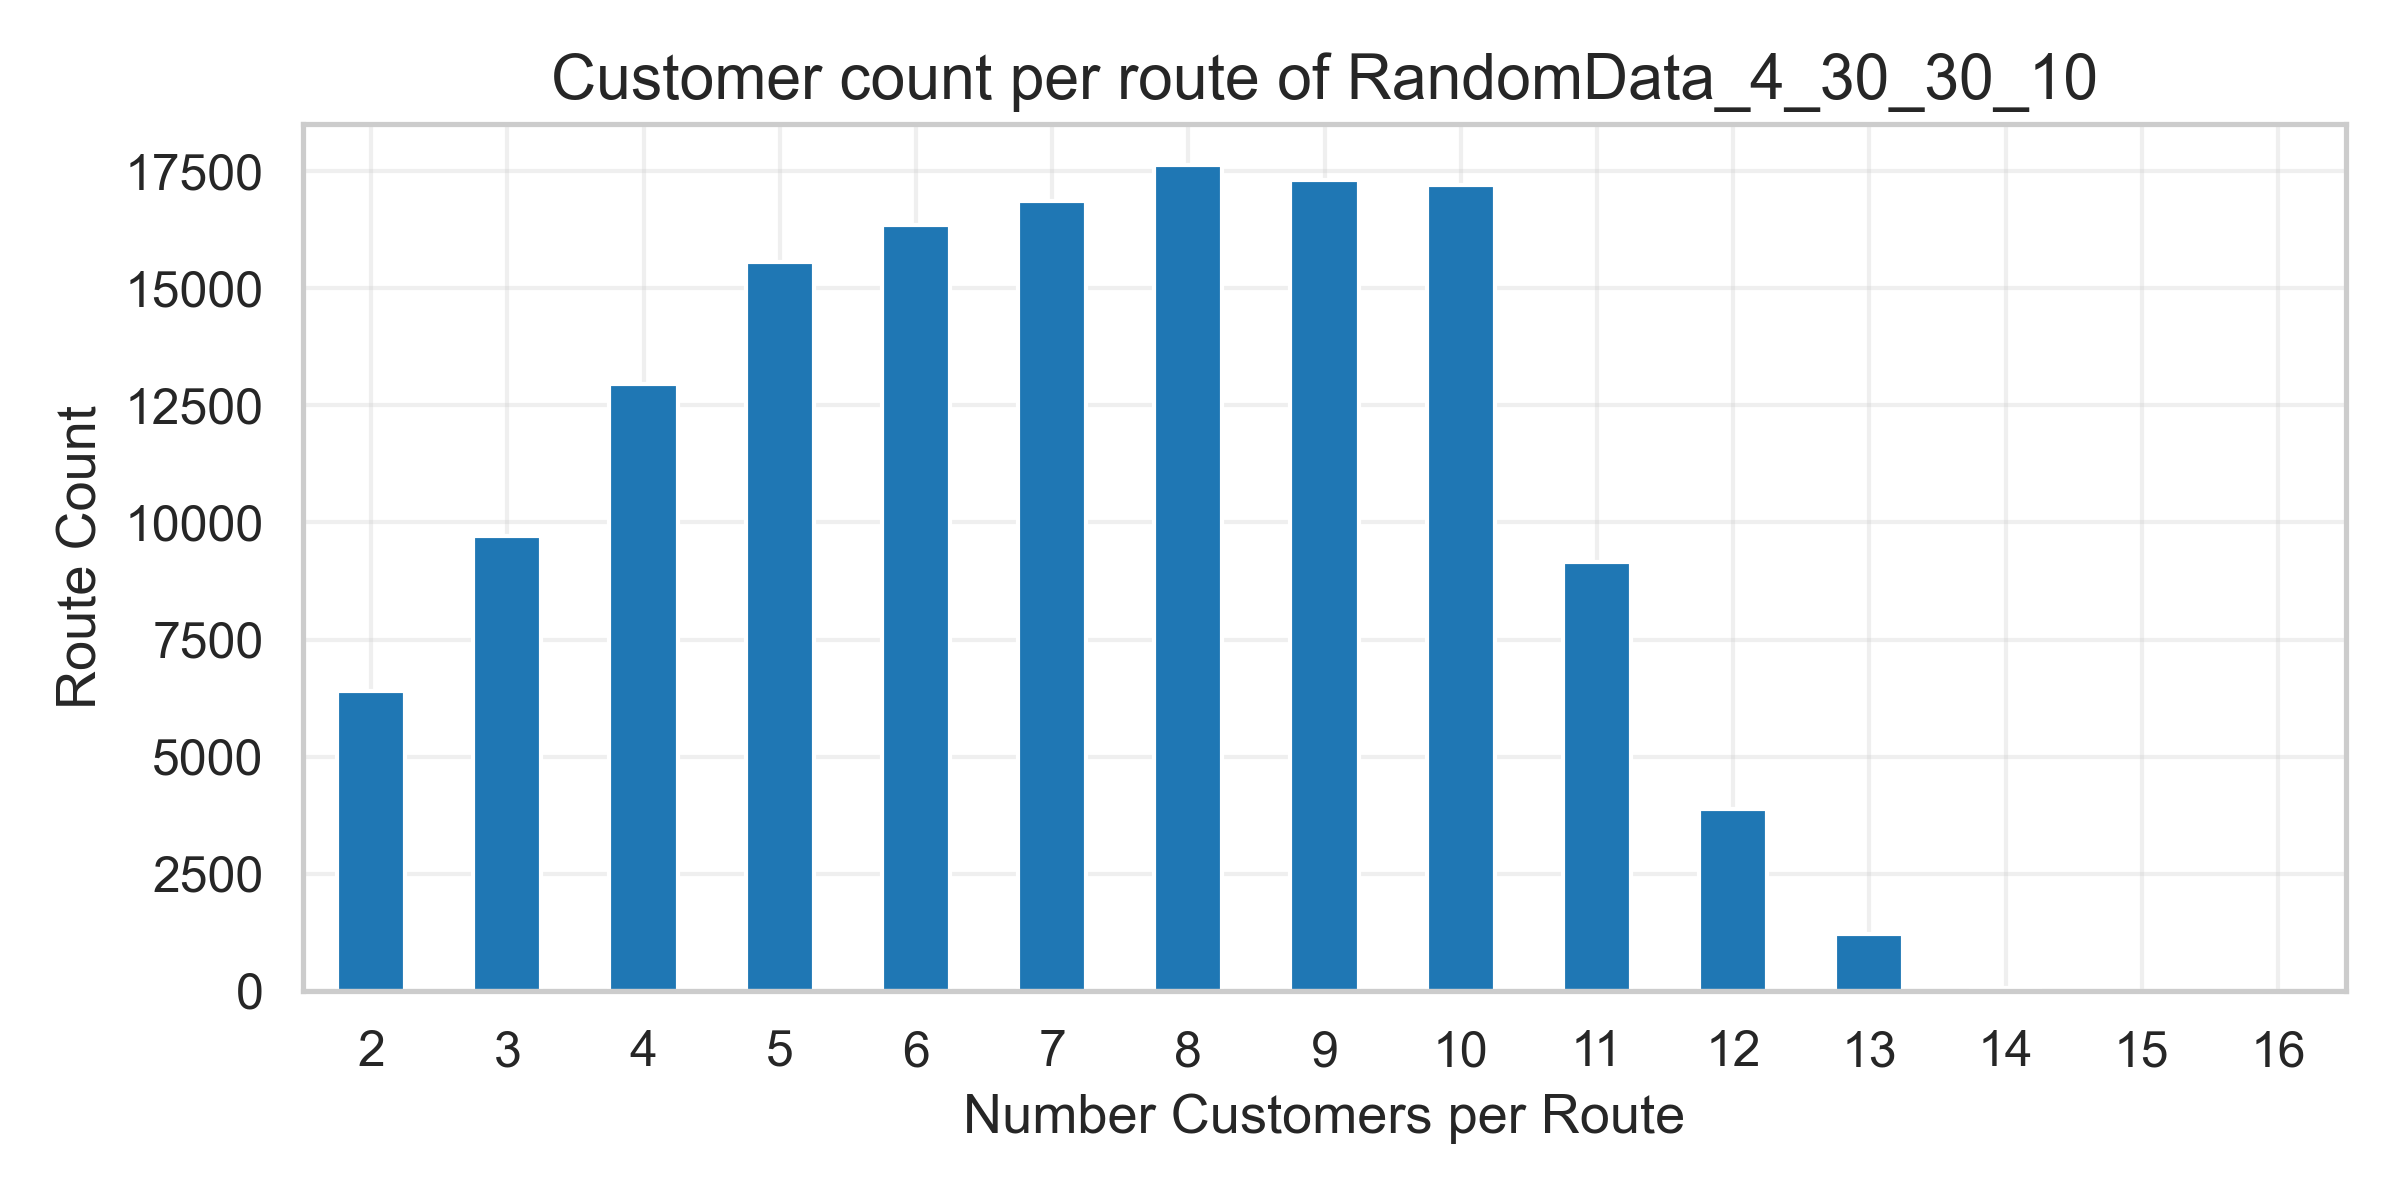
\includegraphics[width=\linewidth]{pictures/dataset_structure/no_cust_plot_RandomData_4_30_30_10.png}
        \caption{Dataset RD-4-30-30-10}
        \label{fig:ds-b-krebs_luf}
    \end{subfigure}
    \caption[Comparison of distribution of route length from random datasets of \krebsADataSetText and \gendreauDataSet.]{Comparison of distribution of route length from random datasets of \krebsADataSetText and \gendreauDataSet. The red vertical line represents the average
        number of customers.}
    \label{fig:route_cust_no_krebs_new}
\end{figure}

\subsubsection{Save retrieval strategy}

Constructing different save strategy datasets was more complex, due to the prolonged run time for the \gls{CP} solver
and undefined behavior for \textit{Invalid} and \textit{Unknown} loading status. The Subsection~\ref{subsec:challenges_krebs_save}
dives deeper in the faced challenges. The results of the modified branch-and-cut results are shown in Table~\ref{tab:bc_results_krebs} and
the following Table~\ref{tab:saved_instances_krebs} presents the created save strategy.
\begin{table}[ht]
    \centering
    \begin{tabular}{l c c c c c c }
        \toprule
        Name           & Sets                 & Routes & Routes Len = 2 & Balance   & Rel. Vol & Rel. Mass \\
        \midrule
        KS-Complete-WS & \multirow{3}{*}{Yes} & 261989 & 220860         & 92.4/7.6  & 0.18     & 0.20      \\
        KS-Trimmed-WS  &                      & 41337  & 208            & 52.1/47.9 & 0.58     & 0.63      \\
        KS-Shrinked-WS &                      & 56962  & 15833          & 65.3/34.7 & 0.43     & 0.48      \\        \midrule
        KS-Complete    & \multirow{3}{*}{No}  & 256786 & 220860         & 94.3/5.7  & 0.16     & 0.19      \\
        KS-Trimmed     &                      & 36134  & 208            & 59.6/40.4 & 0.54     & 0.61      \\
        KS-Shrinked    &                      & 51759  & 15833          & 71.8/28.2 & 0.39     & 0.46      \\

        \bottomrule
    \end{tabular}
    \caption{Save strategy train datsets from \krebsADataSet.}
    \label{tab:saved_instances_krebs}
\end{table}

The "Complete" datasets are dominated by routes with two cutomers, leading to strongly imbalanced datasets. This leaves only
the modified datasets, either shrinked or trimmed, left for model training. But the trimmed dataset will not be used further,
as this datasets can not predict feasible routes with two customers as only infeasible tours for this route length are
present in the dataset.

\subsubsection{Dataset Selection}

To determine the best dataset to be trained, the cross performance metrics of every dataset to all other datasets is compared. However,
as only one save strategy dataset is considered, no cross consolidation results need to be excluded. For all datasets the drop set
DS-50-4 is adopted. Because the model performance was foremost worse due to the big noise of different datasets.

\parbreak

Insert here plot boxplot and tbale of numerical reuslrs how the classification performed.

\parbreak
State final selected model!

\section{Generalize \gendreauDataSetText models}
\label{sec:krebs_data_pretrained_models}

Two alternatives emerge for this variant, on the one hand the best model type and corresponding dataset can be selected from the
computational study of the \gendreauDataSetText (see Section~\ref{sec:comparison_ils_variants}) or on the other the best model type
and dataset is selected by comparing the performance on all five datasets considered in the previous section.
As the second alternative blends the approaches of choosing the same model configuration and adapting the model configuration
to the new dataset, it will only be investigated if the best variant model dataset combinations yield good results for other
\gls{3L-CVRP} datasets. Therefore these condigurations are chosen for the three variants with classifier utilization (see Table~\ref{tab:model_configuration_krebs}).

\begin{table}[ht]
    \centering
    \begin{tabular}{l c c  }
        \toprule
        Variant & Model Type & Dataset      \\
        \midrule
        Filter  & XGB        & RD-4-30-30-6 \\
        SpeedUp & FFNN       & RD-4-30-30-6 \\
        Hybrid  & LR         & RD-4-30-30-8 \\

        \bottomrule
    \end{tabular}
    \caption{Model configuration for generalization of \gendreauDataSetText results.}
    \label{tab:model_configuration_krebs}
\end{table}


\section{Super Cool Results}
\label{sec:results_krebs}
As shown in Section~\ref{app:sec:krebs_computationally_challenges}, the computation of \krebsADataSetText instances comprises
challenges. Therefore, the algorithmic design is changed. As the computation of the start solution takes averagely \textcolor{red}{1000000000000 seconds}
during the B\&C algorithm (20 seconds for the \gendreauDataSetText), much longer running times are needed for the \gls{ILS} algorithm.
Every instance is only run once. Furthermore, the time limit for one instance
is dependent, if the startsolution is given or will be computed during the algorithm. The start solutions are taken from the branch-and-cut
results (see Section~\ref{tab:bc_results_krebs}). Also it is reevaluated, if the parameter UseFilterStartSolution has a positive effect
for instances demanding much longer computation time for the constructive.
\parbreak
Here are the reuslts for the differnt models and combinations of options, to use or not to use the the filter start solution or the given start solution.

\begin{table}[ht]
    \centering
    \begin{tabular}{l c c c }
        \toprule
        Approach               & Startsolution Type & UseFilterStartSolution & Time limit \\
        \midrule
        Krebs training dataset & Given              & False                  & 1 h        \\
        Gendreau model         & ModifiedSavings    & True                   & 2 h        \\
        Gendreau model         & ModifiedSavings    & False                  & 2 h        \\
        \bottomrule
    \end{tabular}
    \caption{Example table.}
\end{table}